


\documentclass[a4paper]{article}
\pdfoutput=1
\usepackage{geometry}
\usepackage{mathtools}
\usepackage{amsmath}
\usepackage{amssymb}
\usepackage{amsthm}
\usepackage[normalem]{ulem}
\usepackage{comment}
\usepackage{env}
\usepackage{enumitem}
\usepackage{multicol}


\newtheorem{protocol}{Protocol}
\newcommand{\Accept}{\mathsf{Accept}}
\newcommand{\Reject}{\mathsf{Reject}}
\newcommand{\Pauli}{\mathcal P}
\newcommand{\Hilbert}{\mathcal H}
\newcommand{\Clifford}{\mathcal C}
\newcommand{\sgn}{\mathrm{sgn}}
\newcommand{\np}{m}
\newcommand{\mCEPS}{\mathcal{C}\text{PS}}
\newcommand{\STAB}{STAB}
\newcommand{\GS}{GS}
\newcommand{\HGS}{HGS}
\newcommand{\pdist}{\mathcal D} % notation for distribution of Pauli measurements for DFE of qubit i (subject to change)
\newcommand{\qdist}{\mu} % notation for qubit choice for DFE (subject to change)
\newcommand{\jdist}{\mathcal D} % joint distribution (subject to change)
\newcommand{\dist}{\mathcal G} % joint distribution (subject to change)
\newcommand{\copyindex}{j}
\newcommand{\qubit}{i}
\renewcommand{\O}{\mathcal O}
\newcommand{\ketbra}[1]{\ket{#1}\!\bra{#1}}
\newcommand{\abs}[1]{\left|#1\right|}
\title{Efficient certification of intractable quantum states with few Pauli measurements}
% \title{Verification of universal quantum computations through single-qubit tomography}

\author{Sami A. Sater, Maxime Garnier, Thierry Martinez, Harold Ollivier, Ulysse Chabaud}
\begin{document}
% \title{Verification of universal quantum computations with single-qubit Pauli measurements}

% \author{Sami Abdul-Sater$^1$, 
% Ulysse Chabaud$^1$, 
% Maxime Garnier$^1$, 
% Thierry Martinez$^1$, 
% Harold Ollivier$^{1}$}
% \affiliation{$^1$ DIENS, Ecole Normale Superieure, 
% PSL University, CNRS, INRIA. first.last@inria.fr}
% \begin{abstract}
% \normalsize
\maketitle
\section{Context and motivation.}  
As quantum technologies mature, 
checking the state produced by a quantum experiment or the result of a quantum computation becomes impractical with standard techniques such as tomography.
Both experimentalists and  clients in cloud-based quantum computing face the common challenge of certifying quantum states and verifying quantum computations.

Verification of quantum computations and certification of quantum states are closely related tasks, particularly for models of computation that proceed by \emph{preparing a specific resource state} and then performing a sequence of adaptive measurements on it to drive the computation. 
Prominent examples include \emph{Measurement-Based Quantum Computation} (MBQC) \cite{RB01one, DKP07measurement, BBDR09measurement} and, even more so, \emph{Magic-State Injection} (MSI) \cite{BK04universal}. 
In the latter, a target resource state is obtained by applying a Clifford circuit to a product of single-qubit states---some of which may be non-stabilizer, or ``magic'', states---followed by adaptive Pauli measurements that realize universal computation. 
Magic-State Injection has become a leading paradigm for \emph{fault-tolerant quantum computation} \cite{DBMA25breaking, G23cleaner, AAAA22suppressing}, as it cleanly separates the easily error-correctable Clifford operations from the costly non-Clifford resources that enable universality.

While verification and certification have been extensively studied in the context of MBQC \cite{TM17verification, TMMM18resource, ZH19efficient, ZH18efficient, LZH23robust}, no efficient protocol is available for the verification of computations based on Magic-State Injection using Pauli measurements—\emph{i.e.}, while requiring the same setup as that used to perform the computation—as we show here.
Direct Fidelity Estimation techniques scale exponentially with the system size \cite{FL11direct, FKMO24learning, SLP11practical}, leaving only fidelity-witnessing-based techniques. Even in that case, the promising result of \cite{HPS24certifying}, which uses Pauli-measurement-based fidelity witnessing to certify “almost all” quantum states, 
and the one of \cite{GHO25few} using single-qubit measurements (possibly non-Pauli) to certify all quantum states, 
crucially rely on a description of the state that is \emph{intractable} for states useful for MSI. 
Indeed, they both assume query access to the target state amplitudes in the computational basis. However, computing the amplitudes of the output state of a quantum circuit is $\#P-$hard in the worst case \cite{A04quantuma, BFNV18quantum}, and in particular for target states relevant for MSI \cite{YJS18quantum}.
This implies that, while potentially being sample-efficient, the protocols \cite{HPS24certifying,GHO25few} would not be time-efficient for all resource states of MSI (unless $P=P^{\#P}$).
This gap is particularly notable given that MSI underlies several practical architectures for scalable, fault-tolerant quantum computing (FTQC) \cite{MGCM25ibm, GSJ24magic}.


\section{Contributions.}
In this paper, we address this gap and introduce a sample-efficient and time-efficient protocol using non-adaptive, single-qubit Pauli measurements for certifying arbitrary quantum states of the form
    $\ket{\Psi} = C\!\left(\bigotimes_{i=1}^n \ket{\psi_i}\right)$,
where $C$ is an $n$-qubit Clifford circuit and $\ket{\psi_i}$ are arbitrary single-qubit states, potentially magic states. 
% \begin{figure}[h]
%     \centering
%     \includegraphics[]{GdR TeQ/figures/CEPS-MSI.pdf}
%     \caption{Structure of a Clifford-enhanced Product State.}
%     \label{fig:CPS}
% \end{figure}
We refer to this family as \emph{Clifford-enhanced Product States} (CPS, inspired by \cite{LHD24quantum}), as it naturally arises by considering an arbitrary $n-$qubit product state and applying an arbitrary Clifford circuit on it, encompassing resource states for Magic-State Injection.
First, we introduce a protocol to certify CPS, 
formulated in the \emph{i.i.d.} setting—\emph{i.e.} when samples are independent and identically distributed. Then, we generalize the approach to the \emph{malicious setting}, where different samples might be correlated. Finally, since Clifford+MSI is a universal model for quantum computing, this provides a natural protocol to efficiently verify any quantum computation using Pauli measurements.

\paragraph{Efficient certification of CPS via fidelity witnessing.}
We provide a protocol that outputs, given a target CPS state and \(N\) copies of a state \(\rho\) (\emph{i.i.d. setting}), a decision of acceptance or rejection of $\rho$ using only single-qubit Pauli measurements sampled from an efficiently computable probability distribution.
Protocol \ref{protocol:certification} (depicted on Fig. \ref{fig:protocol}) is based on fidelity witnessing \cite{CGKM21efficient}: the estimated quantity
$W = 1 - \sum_{i=1}^n (1-F_i)$,
where the $F_i$ are the single-qubit fidelities, is a witness of the global fidelity $F$, in the sense that $W\leq F$.
Consequently, certifying that $W$ is close to one implies a certified lower bound on the true fidelity. The protocol starts by estimating $X:=\sum_i F_i$ then relates it to $W$ via the formula.
Because \(W\) is constructed from the sum of local infidelities, this leads to a completeness condition in which acceptance requires the global fidelity to be \(1-O(\epsilon/n)\), rather than a constant gap as in fidelity estimation (but which would require an exponential amount of samples).

% informal protocol

\begin{protocol}[Certification of CPS (informal)]
\label{protocol:certification}
Let $\ket\Psi = C\bigl(\bigotimes_{i=1}^n\ket{\psi_i}\bigr)$ be the target state and let $\epsilon>0$ be an acceptance threshold.
\begin{enumerate}
    \item For each of the $N$ copies of $\rho$:
    \begin{enumerate}
        \item Sample a qubit index $i$, with higher probability assigned to magic-state qubits.
        \item Sample a single-qubit Pauli observable $P$ from the importance-sampling distribution $\pdist_i$~\cite{FOS24optimal} associated with $\ket{\psi_i}$.
        \item Instead of measuring $P$ on qubit $i$, measure the back-propagated observable
        $C\,P_i\,C^\dagger$ on the prepared $n$-qubit state.
        \label{item:backpropagatino}
    \end{enumerate}
    \item Post-process the measurement outcomes to obtain an estimator $\bar X$ of $\sum_i F_i$.
    \item Compute the fidelity-witness estimator $\bar W$ from $\bar X$. Accept if $\bar W \ge 1-\tfrac23\epsilon$, else reject.
\end{enumerate}
\end{protocol}

% informal theorem
\begin{theorem}[Efficient certification of CPS]
\label{theorem:certification}
        Let $\epsilon,\delta>0$. With the notations of Protocol~\ref{protocol:certification}, assuming $N\ge N_{iid}$ where 
        $N_{iid}\in\O(
                \frac{n^2}{\epsilon^2} \log\left(\frac{1}{\delta}\right)
                )
                \; $
             then Protocol~\ref{protocol:certification} rejects if $F(\rho,\ket\Psi)<1-\epsilon$ and accepts if $F(\rho,\ket\Psi)\ge1-\frac\epsilon{3n}$.
             % \footnote{The constant $\frac13$ is chosen for simplicity and can be replaced by $1-\frac2k$ for any $k\in\mathcal O(1)$ with a constant increase in sample complexity.}, with probability greater than $1-\delta$
    \end{theorem}


% description of the protocol + figure
Back-propagating the Clifford circuit through the measurements is crucial: without it, the protocol would only yield certification of the product state $\bigotimes_i\ket{\psi_i}$. The idea is thus to emulate the uncomputing of $C$—\emph{i.e.} the application of $C^\dagger$—on the received state by changing the Pauli measurement basis, which is done in step \ref{item:backpropagatino}.

\begin{figure}
    \centering
    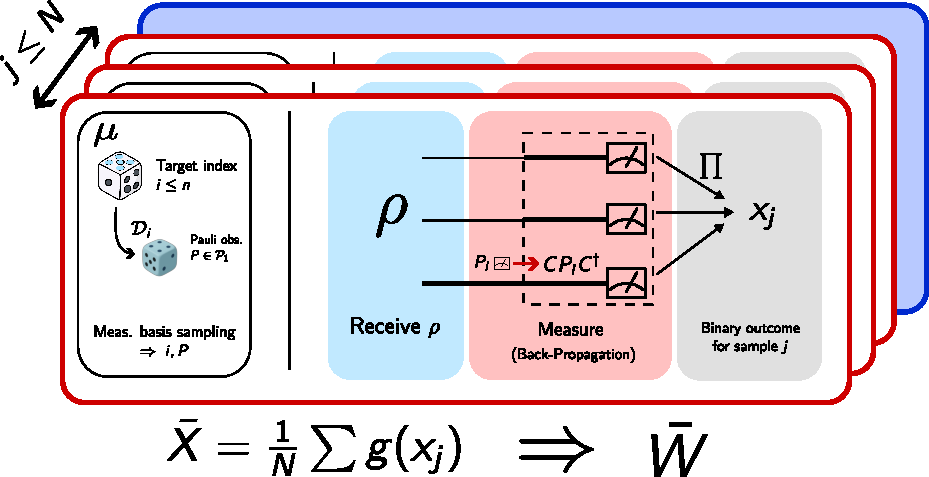
\includegraphics[width=\linewidth]{figures/sf-protocol-ceps.pdf}
    \caption{Visual description of our protocol to certify CPS. The function $g$ denotes a classical post-processing of the outcomes. 
                The samples in red boxes are used for certification, while
                the blue box is a sample that is untouched, left to be used for the computation.}
    \label{fig:protocol}
\end{figure}

\paragraph{In the adversarial scenario.}

By using an improved de Finetti reduction \cite[Theorem 3]{FKMO24learning} for protocols using non-adaptive and incoherent measurements such as ours, CPS can be certified when incoming samples are not i.i.d. copies and might share correlation. The updated protocol consists of increasing the number of samples to $N_{non-iid}$, choosing a random subset of $N_{iid}$ samples on which to apply Protocol \ref{protocol:certification}, discard the $N_{non-iid}-N_{iid}-1$ remaining ones, while one remains for the computation.
The same security guarantees as Theorem \ref{theorem:certification} can be obtained, with $N_{non-iid} \in \tilde\O\left(n^5/(\delta^2\epsilon^6)\right)$.
% \begin{figure}[h]
%     \centering
%     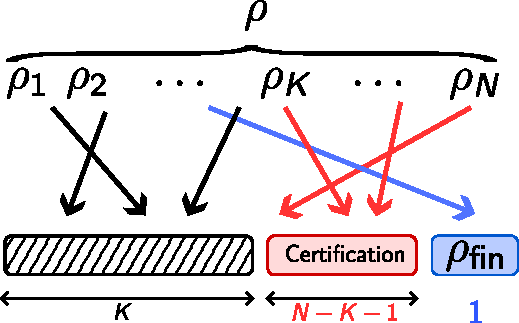
\includegraphics[]{figures/adversarial.pdf}
%     \caption{Caption}
%     \label{fig:placeholder}
% \end{figure}

\paragraph{Verification of universal quantum computation.}
As a corollary of the above, any quantum computation expressed in the Clifford+MSI model admits an associated CPS whose preparation can be efficiently certified via fidelity witnessing. Consequently, conditioned on acceptance of the certification test, any subsequent measurements performed on the remaining copy are guaranteed to be faithful to the ideal computation. This yields an efficient verification procedure for universal quantum computation in the MSI model that relies solely on single-qubit Pauli measurements.


\section{Discussion.}

 This work presents the first efficient solution for the problem of verification of quantum computations expressed in the MSI model relying on single-qubit Pauli measurements only. It indeed stands in contrast to the existing approaches for other models like MBQC (involving Graph states and Hypergraph states verification) or general Pauli-based state certification techniques that requires a description of the quantum state that is $\#P-$hard to obtain in the present case \cite{YJS18quantum}. 
 We expect that this simplicity and scalability will make verification of MSI-based computations an appealing direction for both theoretical study and experimental implementation in near-term quantum platforms.

In particular, it would be interesting to investigate whether the sample complexity in the adversarial setting can be improved using sampling-without-replacement techniques, and whether the class of certifiable states can be broadened by considering back-propagation of observables in other computation models like the coherence-based, rather than the magic-based (Clifford/non-Clifford) framework adopted here.
% \newpage
% we provide to the case where samples might

% We first provide a protocol to efficiently certify CPS~when the received samples are independent and identically distributed (\emph{i.e.} in the \emph{i.i.d.} setting). Then, an immediate corollary from \cite{FKMO24learning} shows how to use the same approach in the \emph{malicious} setting, when different samples might share correlation.
% up to an increase
% % The results are as follow:

% % Our contributions are threefold, where the last two are direct corollary of the first.
% \paragraph{Efficient certification of  CPS}
% The goal of the protocol is to estimate the quantity
% \(\sum_i F_i\), where \(F_i\) denotes the fidelity between the reduced state on qubit \(i\) and the target single-qubit state \(\ket{\psi_i}\).
% This quantity directly determines the fidelity witness through
% \[
% W = 1 - n + n \sum_i F_i .
% \]

% We estimate \(\sum_i F_i\) by Monte--Carlo sampling.
% In each round, we first sample a qubit index \(i\) uniformly at random.
% We then sample a single-qubit Pauli operator \(P\) from the Pauli distribution associated with estimating the fidelity of \(\ket{\psi_i}\).

% Since the target state is obtained by applying a Clifford circuit \(C\) to the product state \(\bigotimes_i \ket{\psi_i}\), we ``back-propagate'' this Pauli through the Clifford:
% instead of measuring \(P\) on qubit \(i\), we measure the conjugated observable \(C P^{(i)} C^\dagger\) on the prepared state.
% This yields an outcome in \(\{\pm 1\}\).

% Repeating this procedure on \(N\) independently prepared copies and averaging the appropriately signed outcomes produces an estimator for \(\sum_i F_i\).
% Plugging this estimate into the expression above gives an estimate of the witness \(W\), which is then compared to a fixed threshold to decide acceptance or rejection.

% \begin{protocol}[Certification of CPS, informal]
%     \label{protocol:certification}
%     Let $\ket\Psi = C\left(\bigotimes_{\qubit=1}^n\ket{\psi_\qubit}\right)$ be the target state to certify and let $\epsilon>0$ be a threshold of acceptance. 
%     \begin{enumerate}
%         \item For each copy:
%         \begin{enumerate}
%             \item Sample efficiently a qubit index $i$
%             \item Sample  single-qubit Pauli $P$ from the distribution $\pdist_i$ from Importance Sampling \cite{FOS24optimal} to estimate fidelity of $\ket{\psi_i}$
%             \item Back-propagate this Pauli through the Clifford:
% instead of measuring \(P\) on qubit \(i\), and measure the conjugated observable \(C P_i C^\dagger\) on the prepared state.
%         \end{enumerate}
        
%         \item Post-process and average the outcomes to get $\bar X$, estimator of $\sum_i F_i$
%         \item Compute estimator of the Fidelity Witness $\bar W$ from $\bar X$. Accept if $\bar W\ge1-\frac23\epsilon$, reject otherwise.
%     \end{enumerate}
% \end{protocol}

%     \begin{theorem}[Efficient certification of CPS]
%             Let $\epsilon,\delta>0$. With the notations of Protocol~\ref{protocol:certification}, assuming $N\ge N_{iid}$ where 
%             \begin{equation}
%             \label{eq:certification:sample iid}
%             N_{iid}\in\O\left(
%                     \frac{n^2}{\epsilon^2} \log\left(\frac{1}{\delta}\right)
%                     \right)
%                     \; ,
%             \end{equation}
%                  then Protocol~\ref{protocol:certification} rejects if $F(\rho,\ket\Psi)<1-\epsilon$ and accepts if $F(\rho,\ket\Psi)\ge1-\frac\epsilon{3n}$\footnote{The constant $\frac13$ is chosen for simplicity and can be replaced by $1-\frac2k$ for any $k\in\mathcal O(1)$ with a constant increase in sample complexity, by replacing the acceptance condition in step 3 of Protocol~\ref{protocol:certification} by $\bar W\ge1-(1-\frac1k)\epsilon$ and setting $\lambda=\frac\epsilon k$ in the proof.}, with probability greater than $1-\delta$.
%         \end{theorem}


% % The most important criteria in their approach are the complexity of the setup and the number of samples required to confidently certify the produced state or computation result.
% % In the literature,
% % this has given rise 
% % to candidate solutions to this problem.
% % % , which can be improved with respect to these criteria.
% % For instance,
% % the state-of-the-art
% % solution using only single-qubit Pauli measurements \cite{HPS24certifying}
% % gives a generic procedure to certify quantum states in which the number of required samples scales in a parameter that depends on the target state. In particular, it is proven to be polynomial in the size of the state for different class of states, such as Haar-random states, graph states, \textit{i.e} classes that are of a particular interest in quantum information processing tasks.

% % allow to verify quantum computations with the same (simple) setup, but the number of samples scales polynomially with the size of the target state, the precise scaling factor depending on the state \cite{HPS25}.

% \medskip
% \paragraph{Related works.}
% On the other hand, more general protocols that aim to certify \textit{any} quantum state have also been studied.
% Traditional techniques such as tomography or Direct Fidelity Estimation scale exponentially with the system size \cite{FL11direct, FOS24optimal, SLP11practical}. Instead general-purpose certification protocols based on fidelity witnessing using Pauli measurements are available for ``almost all'' states~\cite{HPS24certifying} (and even all states when using adaptive measurements~\cite{GHO25few}) but they assume query access to the target state amplitudes in the computational basis. However, computing the amplitudes of the output state of a quantum circuit is $\#P-$hard in the worst case \cite{A04quantuma, BFNV18quantum}, and in particular for target states relevant for MSI \cite{YJS18quantum}. This implies that, while potentially being sample-efficient, the protocols \cite{HPS24certifying,GHO25few} would not be time-efficient for all resource states of MSI (unless $P=P^{\#P}$).

 

% % [Add impact]
% As such, our protocol bridges an important gap, providing an efficient way to certify quantum states in a setting compatible with MSI, where target state amplitudes are classically intractable. It thus offers a practical tool for experimental implementations where Pauli measurements are the natural measurement primitive.



% % \paragraph{Main results.} In this work, we introduce new protocols for certifying another important class of quantum states -- one that enables universal quantum computations -- using only Pauli measurements and where the sample complexity is polynomial in the size of the target state/width of computation.

% \medskip
    
%     \paragraph{Contributions.} 
%     The core contribution of this work is to provide a protocol to certify Clifford-Product States 

%         \begin{protocol}[Certification of CPS]
%             \label{protocol:certification}
%             Let $\ket\Psi = C\left(\bigotimes_{\qubit=1}^n\ket{\psi_\qubit}\right)$ be the target state to certify and let $\epsilon>0$ be a threshold of acceptance. With the notations above, the protocol goes as follows:
%             \begin{enumerate}
%                 \item For each copy $\copyindex\leq N$, sample classically $(\qubit_j, P_j)\sim \pdist$, then measure $C P_j^{(i_j)} C^\dagger$ on $\rho$ (where $P^{(i)}$ denotes the $n$-qubit Pauli operator acting as $P$ on the $i-$th qubit and as identity on all the other qubits), obtaining the outcome $x_j\in\{-1, 1\}$.
%                 \item Compute $\bar X \coloneqq \frac{1}{N}\sum_{\copyindex=1}^N \mathrm{sgn}(\chi_{\psi_{\qubit_j}}(P_j)) \,x_j
%                 $.
%                 \item Output $\bar W\coloneqq 1-n+\np\times \bar X$. Accept if $\bar W\ge1-\frac23\epsilon$, reject otherwise.
%             \end{enumerate}
%         \end{protocol}



    
%     Our contributions are three-fold, and for each we examine the scaling of the number of samples $N$ with respect to the size of the target state/width of the computation $n$, in different scenarios. The security of the protocols is captured by a fidelity error $\varepsilon$ and a failure probability $\delta$.
%     \begin{enumerate}
%         \item We propose a protocol that
%         allows to certify a $n-$qubit quantum state of the form
%         \(
%         \ket{\Psi} = C\left(\bigotimes_{i=1}^n \ket{\psi_i}\right),
%         \)
%         where $C$ is a known Clifford circuit and the $\ket{\psi_i}$ are arbitrary single-qubit states, possibly including magic states, where all samples are \emph{i.i.d}, resulting in $N \sim O(n^3, \log(1/\delta)/\varepsilon^2)$.
%         The main interest of this class  is that together with adaptive single-qubit Pauli measurements, it enables universal quantum computation \cite{BK05}. 
        
%         \item We refine this protocol for specific families of Clifford circuits, showing that the required number of samples becomes quadratic in the computation size: $N \sim O(n^2, \log(1/\delta)/\varepsilon^2)$. 
%         We also show that any quantum computation can be reduced to this setting
%         thus preserving universality.
       
        
%         \item We extend the protocol to the general non-i.i.d.\ setting, in which states might be entangled or correlated across rounds.
%         This version remains efficient and sound under adversarial behavior producing the states.
%         \end{enumerate}

% \medskip

% \paragraph{Techniques.}
% Our protocols rely on an optimal fidelity estimation technique~\cite{FOS24optimal} to estimate the single-qubit fidelities of the pre-Clifford product state, using Pauli measurements on the tested state. 
% This is enabled by the fact that Pauli observables can be efficiently propagated backward through the Clifford circuit $C$ in the Heisenberg picture (in practice equivalent to a classical post-processing of measurement outcomes).
% The resulting local fidelity estimates are then combined into a \emph{robust fidelity witness}~\cite{CGKM21efficient} for the global state, yielding a fidelity error $\varepsilon$ and a failure probability $\delta$. 
% In the third setting, we further show that by applying an optimized quantum de Finetti reduction~\cite[Theorem 3]{FKMO24learning}, the protocol remains sound even against a malicious server employing arbitrary, non-i.i.d.\ strategies across rounds.



% \medskip

% % While robust fidelity witnesses have previously been used in continuous-variable quantum systems, this work demonstrates their first application to discrete-variable systems. 
% % Although originally motivated by experimentalist needs, we show that techniques from quantum state certification also enable efficient verification of quantum computations in cryptographic settings. 
% % Lastly, the required setup involves only single-qubit Pauli measurements, which not only offer practical simplicity but also pave the way for fault-tolerant implementations with limited overhead.
% % % How our protocol compares to \cite{HPS25} regarding this class of states remains an open question.
% % Our certification protocol applies to a large class of target states and is compatible with quantum with magic state injection, a prominent model for realizing universal quantum computations.

% \paragraph{Discussion.}

%  This work presents the first efficient solution for the problem of verification of quantum computations expressed in the MSI model relying on single-qubit Pauli measurements only. It indeed stands in contrast to the existing approaches for other models like MBQC (involving Graph states and Hypergraph states verification) or general Pauli-based state certification techniques that requires a description of the quantum state that is $\#P-$hard to obtain in the present case \cite{YJS18quantum}. 
%  We expect that this simplicity and scalability will make verification of MSI-based computations an appealing direction for both theoretical study and experimental implementation in near-term quantum platforms.

% In particular, it would be interesting to investigate whether the sample complexity in the adversarial setting can be improved using sampling-without-replacement techniques, and whether the class of certifiable states can be broadened by considering back-propagation of observables in other computation models like the coherence-based, rather than the magic-based (Clifford/non-Clifford) framework adopted here.

\newpage
% \begin{multicols}{2}

\bibliographystyle{linksen}
\bibliography{bibliography}
% \end{multicols}

\end{document}
